\documentclass{standalone}

\usepackage{tikz}
\usepackage{pgfplots}
\begin{document}
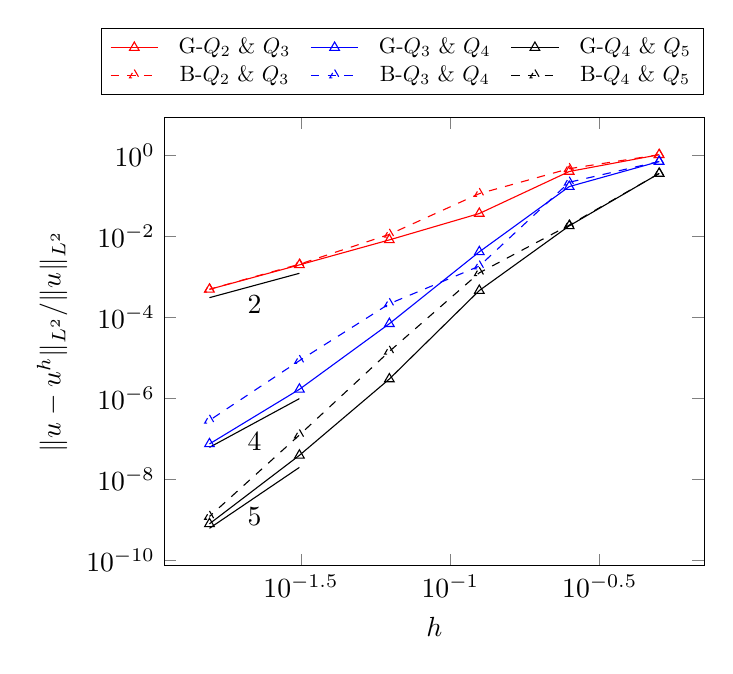
\begin{tikzpicture}
    \begin{loglogaxis}[
        legend columns=3,
    	legend style={at={(1,1.2)}, nodes={scale=0.8, transform shape}, column sep=.2cm},
        xlabel=$h$,
        ylabel=${\|u_{}-u^{h}\|_{L^2}}/{\|u_{}\|_{L^2}}$ 
    ]


    \addplot [color=red,mark=triangle] plot coordinates {

        (.5,    1.02271)
        (.25,   0.393272 )
        (.125,  0.0360061 )
        (.0625,   0.00802147 )
        (0.03125,   0.00193664 )
        (0.015625,  0.00048126 )
    };

    \addplot [color=blue,mark=triangle] plot coordinates {

        (.5,    0.694232)
        (.25,   0.166681)
        (.125,   0.0040645)
        (.0625,   6.81819e-05 )
        (0.03125,   1.6304e-06)
        (0.015625,  7.29714e-08)
    };

    \addplot [color=black,mark=triangle] plot coordinates {

        (.5,    0.351814)
        (.25,   0.0178482)
        (.125,      0.000449695)
        (.0625,     2.92727e-06)
        (0.03125,   3.81391e-08)
        (0.015625,  7.7457e-10 )
    };

    
    \addplot [color=red,mark=triangle, dashed] plot coordinates {

        (.5,    1.02271)
        (.25,   0.461445)
        (.125,   0.111545)
        (.0625,  0.0109794)
        (0.03125,   0.00201306)
        (0.015625,  0.000483481 )
    };

    \addplot [color=blue,mark=triangle, dashed] plot coordinates {

        (.5,    0.694232)
        (.25,   0.213121)
        (.125,      0.00180538)
        (.0625,     0.000212459 )
        (0.03125,   8.31712e-06)
        (0.015625,  2.7879e-07  )
    };

    \addplot [color=black,mark=triangle, dashed] plot coordinates {

        (.5,    0.351814 )
        (.25,   0.0186012)
        (.125,      0.00123195)
        (.0625,     1.40843e-05)
        (0.03125,   1.21223e-07)
        (0.015625,  1.17654e-09 )
    };


    \addplot [black] plot coordinates {

        (0.03125,    0.0012)
        (0.015625,    .0003)
    } node[pos=0.5,anchor=north]{$2$};

    \addplot [black] plot coordinates {

        (0.03125,    9.6000e-07)
        (0.015625,   6e-8)
    } node[pos=0.5,anchor=north]{$4$};

    \addplot [black] plot coordinates {

        (0.03125,    1.9200e-08)
        (0.015625,   6e-10)
    } node[pos=0.5,anchor=north]{$5$};

    \legend{G-$Q_2$ $\&$ $Q_3$\\G-$Q_3$ $\&$ $Q_4$\\G-$Q_4$ $\&$ $Q_5$\\B-$Q_2$ $\&$ $Q_3$\\B-$Q_3$ $\&$ $Q_4$\\B-$Q_4$ $\&$ $Q_5$\\}
    \end{loglogaxis}
\end{tikzpicture}

\end{document}



% 1.02271   0.947573
% 0.393272   0.452374
% 0.0360061   0.150636
% 0.00802147   0.0738313
% 0.00193664   0.0366665
% 0.00048126   0.0183142

% 0.694232   0.675618
% 0.166681   0.29897
% 0.0040645   0.0263881
% 6.81819e-05   0.00385068
% 1.6304e-06   0.000894183
% 7.29714e-08   0.000221005

% 0.351814   0.597089
% 0.0178482   0.069544
% 0.000449695   0.00404805
% 2.92727e-06   0.00023493
% 3.81391e-08   2.65706e-05
% 7.7457e-10   3.25804e-06